\input{/Users/daniel/github/config/preamble-por.sty}
%\input{/Users/daniel/github/config/thms-por.sty}

\begin{document}
\bibliographystyle{alpha}

\begin{minipage}{\textwidth}
	\begin{minipage}{1\textwidth}
		Topologia Diferencial\hfill Daniel González Casanova Azuela
		
		{Prof. Vinicius Ramos\hfill\href{https://github.com/danimalabares/dt}{github.com/danimalabares/dt}}
	\end{minipage}
\end{minipage}\vspace{.2cm}\hrule

\vspace{10pt}
{\huge Lista 3}

\vspace{1em}
\begin{thing1}{Problema 1}\label{prob:1}\leavevmode
Seja \(f: X \to Y\) un difeomorfismo entre duas variedades orientadas conexas. Prove que \(df_x\) preserva orientação para um ponto \(x \in X\) se, e somente se, \(df_x\) preserva orientação para todo ponto \(x \in X\).
\end{thing1}

\begin{proof}\leavevmode
Considere
\begin{align*}
	D: X &\longrightarrow \mathbb{R} \\
	x &\longmapsto \det d_xf
\end{align*}
É uma funcão contínua que nunca pode ser zero. Como é positiva em \(x\), deve ser positiva sempre.
\iffalse
	Pelo teorema da função inversa orientado,  existe uma vizinhança \(U\) de  \(x\) na qual \(\det d_zf\) é positivo para todo \(z \in U\).

Como \(X\) é conexa, podemos ligar \(x\) com qualquer outro ponto \(y \in X\) mediante uma curva \(\gamma\). Pegue em cada ponto \(\gamma(t)\) uma vizinhança na qual \(\det d_{z}f\) é positivo em qualquer ponto \(z\) da vizinhança. Como \(\operatorname{Im}\gamma\) é compacto, temos uma quantidade finita de abertos onde \(\det df\) é positivo.\fi
\end{proof}

\begin{thing1}{Problem 2}\label{prob:2}\leavevmode
Seja \(X\) uma variedade orientável. Prove que a orientação induzida em \(X \times X\) é independente da orientação de \(X\).
\end{thing1}

\begin{proof}\leavevmode
	A orientação de \(X \times X\) está dada como segue: uma base \((\beta_1,\beta_2)\) do espaço tangente \(T_{(x,y)} X \times X\) é orientada se \(\beta_1\) e \(\beta_2\) são bases orientadas de \(X\).

Agora considere a mesma construção usando \(-X\). A base \((\tilde{\beta_1},\tilde{\beta_2})\) de \(-X \times -X\) é orientada se \(\tilde{\beta_1}\) e \(\tilde{\beta_2}\) são bases orientadas de \(-X\).

Porém, é equivalente que \((\beta_1,\beta_2)\) seja orientada em \(X\times X\) e que \((\tilde{\beta_1},\tilde{\beta_2})\) seja orientada em \(-X \times -X\): tanto a transformação que manda \(\beta_1 \mapsto \tilde{\beta_1}\) quanto a transformação que manda \(\beta_2 \mapsto \tilde{\beta_2}\) tem determinante negativo, de modo que a transformação que manda \((\beta_1,\beta_2)\mapsto (\tilde{\beta_1},\tilde{\beta_2})\) tem determinante positivo!
\end{proof}

\begin{thing1}{Problem 3}\label{prob:3}\leavevmode
Prove que \(\mathsf{SO}(n)\) é uma variedade orientável e calcule a sua dimensão. Usando teoria da interseção prove que \(\chi(\mathsf{SO}(n))=0\).
\end{thing1}

\begin{proof}\leavevmode
	First notice that \(\mathsf{SO}(n)\) is one of the connected components of \(\mathsf{O}(n)\). Indeed, \(\mathsf{SO}(n)=\det^{-1}(1)\) for the submersion \(\det:\mathsf{O}(n)\to \{\pm 1\}\), making into a codimension-0 submanifold of  \(\mathsf{O}(n)\) since \(\dim \{\pm 1\}=0\). This means that computing the dimension of \(\mathsf{SO}(n)\) is the same as computing the dimension of \(\mathsf{O}(n)\).

	Now observe that a matrix in \(\mathsf{O}(n)\) is the same as an orthonormal frame of \(\mathbb{R}^n\): the column vectors of any  \(A \in \mathsf{O}(n)\) unitary and mutually orthogonal since \(A A ^{\mathbf{T}}=\operatorname{Id}\) says \(\sum_{k}a_{ik}a_{jk}=\delta_{ij}\) for every \(i,j\). 

	We can compute the dimension of \(\mathsf{O}(n)\) as follows. Take a vector \(v_1\) in \(S^{n-1}\), then a unitary vector in the orthogonal complement of  \(v_1\), i.e. a vector in \(S^{n-2}\), and so on until we choose either of the two vectors in \(S^0\). This means that we are choosing points in \(S^{n-1}\times S^{n-2} \times \ldots \times S^0\), which gives \(\dim \mathsf{O}(n)=\sum_{i=0}^{n-1}i\). It is well known that this number is \(\frac{n(n-1)}{2}\).

	To orient \(\mathsf{SO}(n)\) just notice that it acts on itself homogeneously (by orientation-preserving diffeomorphisms). Taking a basis at the identity matrix and moving it around our manifold using this action generates a smooth global choice of local orientations; i.e. a global orientation.

	The fact that \(\chi(\mathsf{SO}(n))=0\) is immediate from the fact that its tangent bundle is trivial: there is a nowhere vanishing vector field (the orbit of any nonzero vector), giving the result by Poincaré-Hopf theorem.
\iffalse
	\(\mathsf{SL}(n)\) is \(\det^{-1}(1)\) for \(\det:\mathsf{GL}(n)\to \mathbb{R}\). And \(\mathsf{O}(n)\) is \(F^{-1}(\operatorname{Id})\) for \(F: \mathsf{GL}(n)\to \mathsf{GL}(n)\), \(A \mapsto  A A^{\mathbf{T}}\). And then \(\mathsf{SO}(n)=\mathsf{SL}(n)\cap \mathsf{O}(n)\).

To compute the dimension of \(\mathsf{SO}(n)\) consider the embedding \(\mathsf{O}(n)\hookrightarrow \mathsf{GL}(n)\). If \(\mathsf{O}(n)\pitchfork \mathsf{SL}(n)\) we get that \(\mathsf{SO}(n)\) has the same codimension inside \(\mathsf{O}(n)\) as the codimension of \(\mathsf{SL}(n)\) inside \(\mathsf{GL}(n)\), the latter being 1 since it is a level-set of a real valued function. {\color{2}But what is the dimension of \(\mathsf{O}(n)\)?}

To give \(\mathsf{SO}(n)\) an orientation we can use the preimage orientation. That is\fi
\end{proof}

\begin{thing1}{Problem 4}\label{prob:4}\leavevmode
Seja \(\Sigma\) uma superfície de gênero \(g\). Construa um campo vetorial em \(\Sigma\) com um único zero de índice \(2-2g\).
\end{thing1}

\begin{proof}[Solution]\leavevmode
Primeiro note que é suficiente construir um campo vetorial com um único zero, já que pelo teorema do índice de Hopf ele necessariamente vai ter índice \(2-2g=\chi(\Sigma)\). (Um modo de comprovar que essa é a característica de Euler de \(\Sigma\) é usando o campo gradiente da função altura, que tem dois zeros de índice 2 e \(2g\) zeros de índice \(-1\).)

Para constuir um campo vetorial com um único zero usarei ideas de \href{https://math.stackexchange.com/questions/1453942/existence-of-a-vector-field-with-one-singularity-on-a-surface}{StackExchange}.

Sabemos que \(\Sigma\) pode ser vista como um polígono com certas identificações no bordo. Podemos dar uma decomposição simplicial dele simplesmente botando um vértice no centro do polígono e as aristas que ligam os vértices do polígono com o centro. Ussando o campo vetorial para triangulações discutido em aula,
\begin{figure}[H]
	\centering
	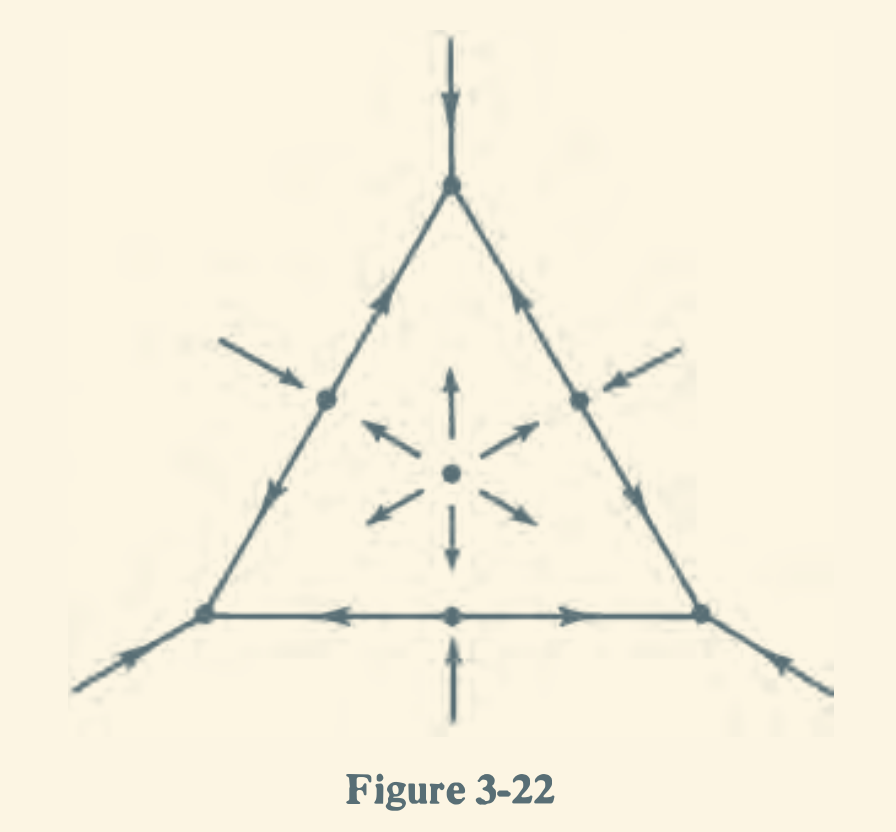
\includegraphics[width=0.3\textwidth]{fig1.png}
\end{figure}
obtemos um campo vetorial em \(\Sigma\) com uma quantidade finita de zeros.

A ideia é construir um grafo conexo em \(\Sigma\) cujos vértices sejam os zeros do campo, e que não tenha ciclos i.e. uma árvore. Desse jeito, uma vizinhança tubular do grafo é homeomorfa a um disco, e a restrição do campo a esse disco não tem zeros no bordo. Daí conseguirmos perturbar o campo ussando à ``Adaptação do truque de Alexander":

\begin{lemma}\leavevmode
Se \(v\) é um campo vetorial suave em \(D^2\) sem zeros no bordo, existe outro campo vetorial suave com um único zero que coincide com \(v\) no bordo.
\end{lemma}

\begin{proof}[Prova do lema]\leavevmode
Como \(v\) não tem zeros no bordo (e o nosso \(v\) na verdade tem uma quantidade finita de zeros) podemos pegar um \(\varepsilon<1\) tal que os zeros de \(v\) estão na bola \(B_\varepsilon\). Daí pegamos uma bump function \(\rho\) que tenha um único zero em zero e seja constante 1 fora de \(B_\varepsilon\).

Então defina
\[w(r,\theta)=\begin{cases}
	v(r,\theta)\qquad &r \geq \varepsilon \\
	\rho(r)v(\varepsilon,\theta)\qquad &r \leq \varepsilon
\end{cases}\]
\end{proof}

\end{proof}

\begin{thing1}{Problem 5}\label{prob:5}\leavevmode
Seja \(A\) uma matriz de \(n \times n\) com coeficientes inteiros e seja \(f:\mathbb{R}^2/\mathbb{Z}^2 \to \mathbb{R}^2/\mathbb{Z}^2\) tal que \(f(x)=Ax\). Calcule o grau de \(f\).
\end{thing1}

\begin{proof}\leavevmode
	To compute the degree of \(f \) it's enough to compute the number of preimages of \([0] \in \mathbb{R}^n/\mathbb{Z}^n\). To do this consider the fundamental domain \([0,1)^n\) and map it with \(A\) to  \(\mathbb{R}^n\). When we take the quotient, all the points with integer coordinates will be glued together in the class \([0]\). I.e. we are looking for the number of points with integer coordinates in \(P:=A\Big( [0,1)^n \Big)\).

	I claim that this number is the volume of \(P\), i.e. the determinant of  \(A\). While this is intuitively clear, I was unable to produce a formal proof.

	\begin{figure}[H]
		\centering
		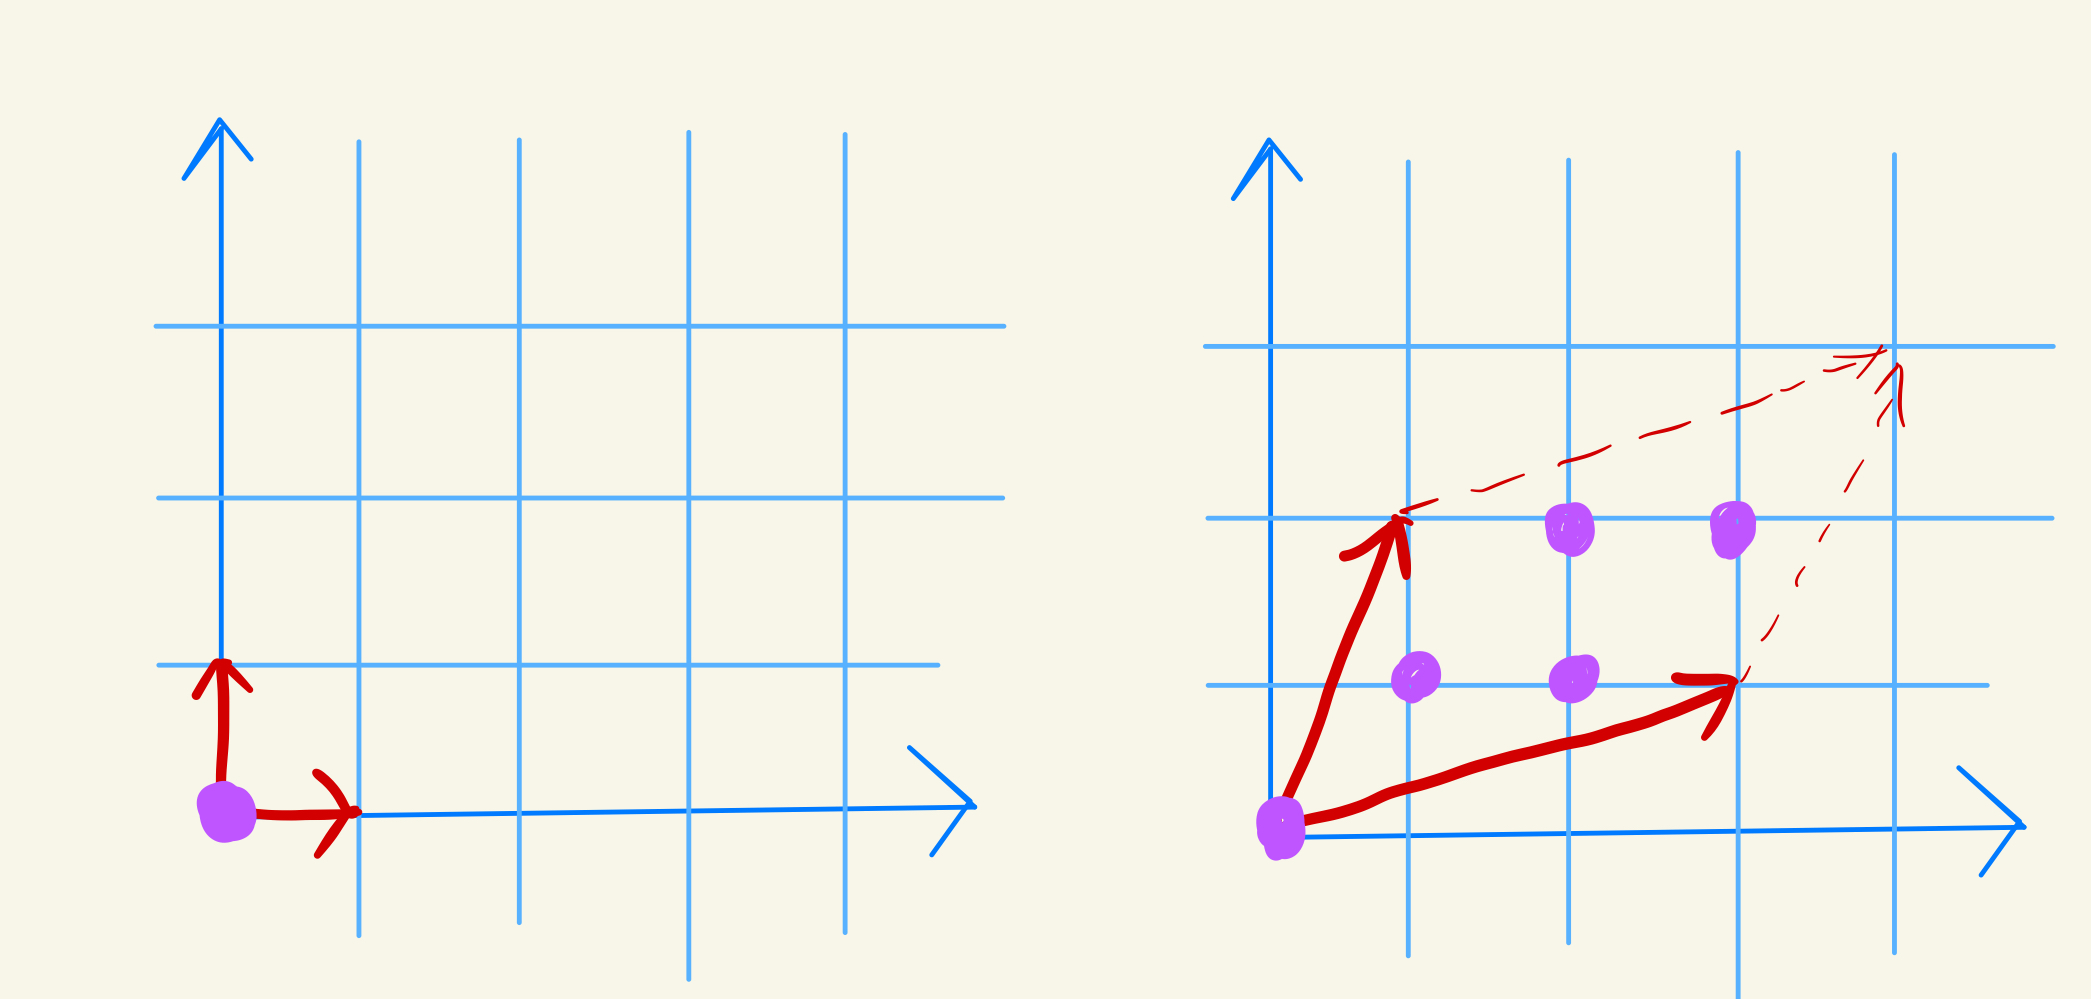
\includegraphics[width=0.7\textwidth]{fig2}
		\caption*{Example for \(A=\begin{pmatrix}3&1\\ 1&2\end{pmatrix}\), with determinant \(5\)}
	\end{figure}
\iffalse

	To see why consider the case of dimension 2. We may assume that the image of \(e_1\) is a vector in the \(x\) axis using a rotation (which preserves the volume of \(P\) \textit{and} the ammount of integer points inside \(P\)). The number of integer points inside \(P\) after rotating is simply the product of the lengths of \(Ae_1\) and \(Ae_2\):


	This product is \(\det A\)


	the case of two dimensions. First use an isometry to assume that one of the sides of \(P\) is in the \(x\) axis. Then consider the map that projects the other side of \(P\) to the \(y\) axis, mapping \(P\) to a rectangle

	the area of \(P\) is the same as the area of the rectangle we obtain when projecting the side
	
	First consider the case for \(n=1\). Take the class \([0] \in \mathbb{R}/\mathbb{Z}\) and let's check how many preimages it has in the fundamental domain \([0,1) \subset \mathbb{R}\). Our matrix \(A\) is only a number, say \(a\). So we have \(ax \in [0]=\{0+n:n \in \mathbb{Z}\}\). This just says \(ax \in \mathbb{Z}\) which happens when \(x\) is a rational number with  denominator \(a\), and there's  \(|a|\) such numbers in \([0,1)\).

	Now for the case  \(n=2\) suppose \(A=\begin{pmatrix} a & b\\c & d \end{pmatrix} \), and let's look for points \(\vec{x}=(x,y) \in [0,1)^2\) such that \(A\vec{x} \in [\vec{0}]=\mathbb{Z}^2\). This means that
	\[A \vec{x}=\begin{pmatrix} a & b\\c & d \end{pmatrix} \begin{pmatrix} x\\y \end{pmatrix} =\begin{pmatrix} ax+by\\cx+dy \end{pmatrix} \in \mathbb{Z}^2.\]
	 Substracting these two conditions (that \(ax+by \in \mathbb{Z}\) and that \(cx+dy \in \mathbb{Z}\)) we obtain that
	 \[x(a-c) + y(b-d) \in \mathbb{Z}\]
	Suppose for a second that \(y=0\): we go back to a case similar to the 1-dimensional, namely there are \(|a-c|\) solutions. The same works whenever \(y(b-d) \in \mathbb{Z}\), for which there are \(|b-d|\) choices. So there's \(|a-c||b-d|\) solutions.
\fi
\end{proof}


\begin{thing1}{Problem 6}\label{prob:6}\leavevmode
Prove que \(\mathbb{R}P^{2n+1}\) é orientável e que \(\mathbb{R}P^{2n}\) não é orientável.
\end{thing1}

\begin{proof}\leavevmode
	First notice that \(-\operatorname{Id}\) preserves orientation iff \(n\) is odd. This map is a composition of \(n\) reflections, one about every axis of \(\mathbb{R}^{n+1}\supset S^n\). Each of these reflections is orientation-reversing, and composing a map with an orientation-reversing map reverses orientation by the chain rule.

	Now recall that \(\mathbb{R}P^{n}=S^{n}/-\operatorname{Id}\). Suppose \(\mathbb{R}P^{n}\) is orientable, so that the quotient map is orientation-preserving since it is a submersion: the determinant of its differential is a nowhere-zero continuous function on a connected manifold, so it cannot be positive somewhere and negative elsewhere.

	Choose an oriented basis of the tangent space of \(\mathbb{R}P^{n}\) at \([e_1]\). Pull back the basis using quotient map, this produces a basis at each of the preimages, namely \(e_1\) and \(-e_1\). These two bases must be in the same orientation of \(S^{n}\) since the quotient map is orientation-preserving and they are mapped to the same basis in the quotient. However, this only happens when \(-\operatorname{Id}\) is orientation-preserving.
\end{proof}



\end{document}
